Data reduction is integral to geoscience from  Babylonian astronomers through the Mars rovers to facilitate transfer and analysis of data.
Space exploration mission science is constrained by dataflow driven duty cycling limitations on both the space platforms \citep{kurth1979} and the ground stations \citep{deutsch1982}.
Computing advances quantified in section~\ref{sec:prochistory} brought robust computing and storage solutions to the commercial market.
These advances have trickled down to radiation-hard processors, memory and storage sufficient for autonomous driving of Mars rovers \citep{woods2014}.
Novel radio signal processing techniques have enabled rescue of otherwise lost missions and exploration beyond Neptune \citep{deboy2004,haskins2007}.
Much of the data from the 1995 Galileo Jupiter encounter was saved via novel data compression \citep{cheung1996} and fortuitous overprovisioning of storage (\unit[110]{MByte} tape, \unit[192]{kByte} RAM) \citep{marr1994} connected to the late 1970s 1802 CPUs \citep{thomas1980}. 
The lossy compression overcome a 10000:1 reduction in planned downlink data bandwidth, reverting from what was to be a \unit[134.4]{kbps} downlink \citep{layland1990} to \unit[16]{bps} \citep{beyer1996}, allowing Galileo to usefully serve at Jupiter from 1995 to 2003.
The combination of robust embedded computers, storage and wireless connectivity enables a new generation of remote, autonomous geoscience observatories via appropriately designed data reduction algorithms.

Virtually everywhere above ground on earth is covered by ``unlimited'' usage satellite data connectivity at tractable cost.
Iridium unlimited data usage is currently \$125/month\footnote{Pricing for Iridium GO! via \url{http://www.bluecosmo.com/iridium-go/rate-plans}} at \unit[2.4]{kbps}, with future speeds up to \unit[128]{kbps} and essentially global coverage.
Covering the northern auroral oval and beyond, unlimited usage satellite data from Globalstar is currently \$150/month at \unit[9.6]{kbps}, with future speeds up to \unit[256]{kbps} \citep{globalstar2015}.
The Globalstar data rate with coverage area shown in Figure~\ref{fig:globalstar} is similar to that experienced with the DMC instrument in section~\ref{sec:dmc}.
\begin{figure}
    \includegraphics[width=\linewidth]{gfx/voice-coverage_map_lg_w_homezone_oct31_14}
    \caption{Current Globalstar satellite data coverage area in yellow and gray.}\label{fig:globalstar}
\end{figure}
Terrestrial mobile data networks generally have higher data bandwidth than satellite.
Due to petrochemical extraction and other human activity, 4G networks are extending across the auroral zone.
Even the slopes and summit of Mt.\ Everest have 4G cellular service \citep{oberhaus2016}. 
%since 2011, with Everest base camp having satellite connectivity since 1996.
Cubesats are forming networks to relay data on orbit for terrestrial downlink \citep{parham2016}.
Commercial magnetometers aboard he Iridium 66~satellite constellation have been turned into the AMPERE observatory \citep{waters2001}.
AMPERE creates a global current map relevant to auroral precipitation using geomagnetic spherical harmonic analysis introduced by \citet{gauss1839}.

As a practical matter for geoscience imaging systems, data rates less than about \unit[4.8]{kbps} are useful for system control and low resolution preview data, while data rates above \unit[9.6]{kbps} become practical for curated retrieval of limited data sets.
Historically this has meant taking a picture of the aurora perhaps once per minute since there was no means of storing or transmitting vast amounts of high speed video--a problem from 1900 through the developments of this chapter started in 2012.
The experience with the DMC instrument in Greenland and isolated deployments for the HiST system using 4G wireless data have shown the utility of automated data reduction algorithms for auroral research.
With the algorithms developed in this chapter, auroral and geoscience radar researchers can record high speed data and store/download interesting segments of data remotely.

For geospace data in general and in particular for auroral video observatories, significant portions of data collected will be of little value relative to the cost of transporting the data.
Multiple generations of geospace satellites have duty cycled observations to conserve power, storage, and downlink bandwidth.
While miniature instrument technologies and streaming data bandwidths have  advanced to the point where cameras and radars covering the entire MF/HF band fit into a 3U Cubesat \citep{knapp2016}, data downlinks are strained by the amount of data collected.
Most contemporary high speed auroral imaging systems are severely limited by duty cycle to avoid overflowing their on-site data storage \citep{fukuda2016}.

Distributed geospace sensors, particularly dense arrays with dozens or hundreds of nodes \citep{pankratius2014}, can benefit from on-site data reduction.
Even though 4G connectivity in the northern auroral oval (approximately $60^\circ$N to $70^\circ$N) continues to expand, the coverage is generally spotty due to terrain and great inter-tower distances.
Figure~\ref{fig:gci} is an example of the spotty coverage endemic to rural areas due to low tower density and vast distances with terrain.
\begin{figure}\centering
	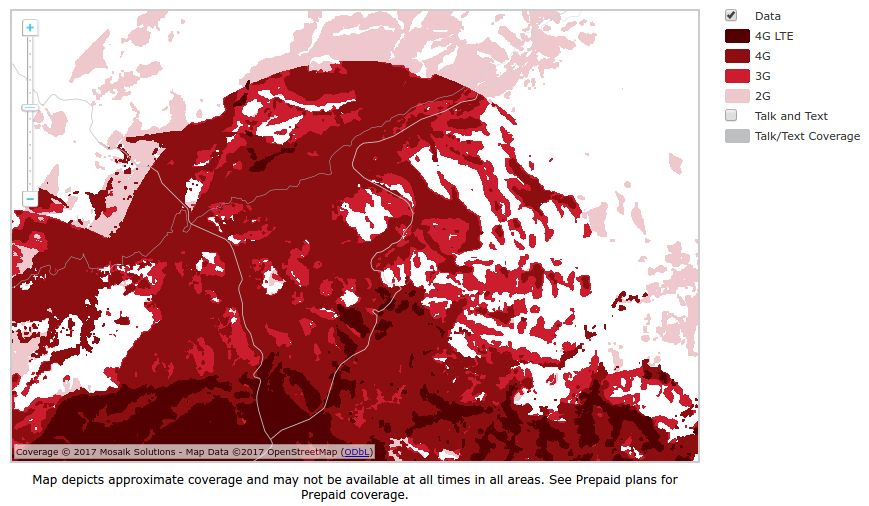
\includegraphics[width=\linewidth,trim=0 45 0 0,clip]{gfx/gci4g-pfrr}
	\caption{GCI wireless data coverage near Poker Flat Research Range. Map is roughly \unit[30]{km} in vertical extent.}\label{fig:gci}
\end{figure}
Weak wireless signals directly imply reduced data speed via the Shannon-Hartley theorem \citep{nyquist1924,hartley1928,shannon1948a,shannon1948b,lee1990}
\begin{equation}\label{eq:shannon}
C = B \log_2\left(1+\frac{S}{N}\right)
\end{equation}
where $C$ is the channel capacity in bits/s, $B$ is the channel bandwidth in Hz, $N$ is the noise power in $B$ and $S$ is the signal power. 
Software defined radio sensors for HF, GPS and other radar applications generate up to the order of a terabyte of data per day, while EMCCD and sCMOS cameras used for auroral and airglow observations generate several terabytes per night \citep{hirsch2016}.
Assuming unlimited data plans (2016 prices $\sim$ \$200/month) and future \unit[1]{Gbps} radio data bandwidth, the avalanche of data from hundreds of sensors must be sifted through at some point in the system lifetime.

Where sufficient local computing power (both CPU and watts) exists, it is typically advantageous to reduce the data on-site before transmitting to a central repository.
For those situations where it is desirable to retain all data to allow for discovery of an unknown, as yet uncharacterized phenomenon, data reduction techniques are still essential for tagging known event types.
In general, remote geoscience observatories require on-site and/or fog computing due to constrained storage and data bandwidth to the outside world.
The problem of high-bandwidth sensors with constrained connections is common in remote sensing system, including smart transportation \citep{hou2016}.
A common sparse messaging format allows telling groups of sensors to store segments of high resolution data without processing the data at each and every node all the time.
An HDF5 format file with the nightly triggering record from a high-power sensor node is less than \unit[25]{kB} for a 12 hour period, a size readily relayed over a \unit[1.2]{kbps} radio link.
Integrated radio modules with antennas cost about \$50 and use world-wide license-free frequencies near \unit[900]{MHz} with approximately \unit[1]{km} range between nodes.
By \eqref{eq:shannon}, using larger directional antennas allows longer range or higher data rates.
An example of the utility of such a system is a dense network of high speed magnetometers with kilometer grid spacing \citep{raeder2016}, where to conserve solar-charged batteries, recording and/or relaying of data only occurs on all nodes during auroral events.

A large subclass of geospace instruments are designed to observe infrequent, irregularly occurring events.
Instruments designed to capture only the strongest events (typically making a sensor cheaper) will cost much more in terms of lost sensing opportunities and wasted energy and exergy.
Instruments are often a bit overdesigned in terms of sensitivity and dynamic range to allow for discovery of new phenomena.
The slight Arecibo overdesign for plasma characterization \citep{farley2012} allowed the radar to receive gyro-line plasma emissions. 
Arecibo's increased SNR is also used for planetary body characterization and asteroid imaging to complement facilities such as the shorter wavelength Goldstone Radar \citep{slade2011}.
Higher instrument sensitivity may bring new discoveries via newly seen weak signals, which need to be sifted through for events of interest.

For auroral targets specifically, several attributes of the targets have been exploited.
\citet{rao2014} used RGB-transformed color as an essential component of auroral detection at multiple stages.
For reasons stated in chapter~\ref{chapter:sim}, only grayscale video is available from HiST.
Several machine learning approaches have been used for slow-acquiring all-sky cameras that collect as many frames in a year as HiST does for each camera per night \citep{mikka2005}.
Decomposition methods have been applied to high-SNR video as part of an effort to create a search engine for auroral forms \citep{mikka2002}.
These methods are not suitable for the high speed auroral video generated by the DMC and HiST instruments.

DMC and HiST need a fast auroral detection algorithm to wade through terabytes of data per camera per night. 
Unlike previous efforts, the dynamic structured aurora discriminator (DSAD) algorithm does not necessarily need to make a final classification of auroral type, particularly when used with the HiST inversion algorithm described in chapter~\ref{chapter:sim}.
The DSAD task of interest is detecting fine spatiotemporal auroral features, which have distinct characteristics that are exploited via a collective behavior algorithm developed for this thesis.
A modified version of the DSAD algorithm has been extended to passive ionospheric radar, described in appendix~\ref{chapter:passive}.
Another modified DSAD application is demonstrated for the HF top-sounding radar MARSIS exploring the Martian ionosphere in appendix~\ref{chapter:marsis}.

\section{Auroral Data Processing Background}\label{sec:prochistory}
Quantitative auroral observations rely on large datasets collected at multiple locations over an extended period of time (see section~\ref{sec:obshistory}).
A general algorithm for the processing of auroral data is depicted in Figure~\ref{fig:genalgo}.
\begin{figure}\centering 
    %the \par is necessary after each text to make the \baselineskip take effect
    \begin{tikzpicture}[node distance=1.5cm, auto]
    
    \node (in) [startstop,text width=2cm] {streaming data frames \par};
    
    \node (detect) [compute, right of=in,text width=3cm,xshift=2cm] { Detect Auroral Morphology \par };
    
    \node (reduce) [process, right of=detect, text width=3cm,xshift=2.5cm] { Dimensionality Reduction \par };

	\node (store) [startstop, right of=reduce,text width=3cm,xshift=2.5cm] { store/transmit tabulated data \par};
    
    \draw[arrow] (in) -- (detect);
    \draw[arrow] (detect) -- (reduce);
    \draw[arrow] (reduce) -- (store);

    
    \end{tikzpicture}
    
    \caption{Block diagram of DSAD algorithm.}
    \label{fig:genalgo}
\end{figure}
%Tables of auroral activity versus time and location were extensively compiled in the 1700s (see section~\ref{sec:historyaurora}), a simple but highly lossy form of data reduction.
The technology necessary for quantitative spatiotemporal observations on sub-second timescales necessary for understanding structured aurora evolved throughout the twentieth century via several technological advances:
\begin{enumerate}
    \item quality spectrum resolution: \citep{sykora1901} high resolution, sensitive auroral spectrum obtained with several hour exposures % to day-long
    \item stable fast optics: \citep{stormer1932} auroral images capturing from UV to IR with half-second exposure, with hundreds of cameras manufactured and globally distributed for IPY 1932 (see section~\ref{sec:obshistory}).
    \item stable stopband filters: \citep{rayleigh1924} using repeatable Kodak Wratten filter arrangement allowed blocking undesired emissions while maximizing observed brightness, in a replicable, global transportable system.
    \item fast energy spectrum of precipitating particles: \citep{sharp1965} \unit[8]{ms} cadence broadband differential number flux, revealed fine spatiotemporal structure and that electrons were responsible for structured aurora
\end{enumerate} 
Several more developments enabling digital computer processing of video were necessary to enable the millisecond timescale auroral observations of the twenty-first century:
\begin{enumerate}[resume]
    \item digital cameras: CCD technology that came to market in the early 1970s and subsequent market availability of intensified CCD (iCCD), sCMOS, and EMCCD imagers rugged and inexpensive enough for global shipment and reuse by the early 2000s.
    \item large, fast, durable portable storage media: by 2008 beginning to be adequate for storing one night's data and by 2009 \unit[2]{TB} HDDs available for \$300 \citep{first2tb} capable of two nights' data.
\end{enumerate}
Corporate termination of scientific film production in the mid-1990s \citep{malin1993} combined with the rise of wider dynamic range, high sensitivity digital scientific cameras accelerated the switchover from analog to digital imaging.
ISR also benefited from the advances in computer technology to process 4096 antenna elements worth of reduced streaming data.
High-power microwave modules and associated technology for electrically steerable phased array radar \citep{valentic2013} and broadband software defined radio \citep{vierinen2016} are additional vital developments necessary for quantitative analysis of NEIALs vis-à-vis Alfvénic aurora.

\subsection{Computing Hardware Relevant to Auroral Data Processing}\label{sec:currentpc}
%  = 1.27 TB / 12 hour night
Since each EMCCD camera used in HiST generates on the order of
\begin{equation}\label{eq:mbsec}
    \unit[512^2]{pixels} \times \unit[2]{bytes/pixel} \times \unit[56]{frames/s} \sim \unit[29.4]{MB/s} 
\end{equation}
\begin{equation}
     \unit[(29.4\times 3600)]{frames/hour} \times \unit[10]{hours} \sim \unit[1.1]{TB/night}
\end{equation}
an internal HDD with at least \unit[1.5]{TB} of storage is necessary to avoid excessive fragmentation upon writing each night's data.
Fragmentation is relatively benign on SSD but for HDD the large additional mechanical seek time from fragmentation can cause greater than 90\% reduction in read/write rate, which is problematic for auroral video.
Empirically we have found that keeping the HDD with at least 5\% free space using exFAT formatting \citep{munegowda2014exfat} has avoided write speed problems due to fragmentation.
By \eqref{eq:mbsec} and lab experiments conducted during lab verification of DMC and HiST phase 1, the HDD should have at least \unit[75]{MB/s} sustained write speed, giving margin for nonidealities and congestion involved in sustained sequential writes to avoid overflowing the RAM buffer and thereby losing data.
Sustained HDD write speed specifications may be actually given as an average or N\textsuperscript{th} percentile, and also depends on format and operating system overhead, so at least a cursory lab verification before buying several HDD is well-justified.
An example of lesser real-world performance versus spec sheet was given by \citet{hddrealworld}, in accord with experience in DMC lab verification.
Real USB~2.0 HDD are limited to about \unit[40]{MB/s} sustained sequential write speed.
Putting the same modern HDD into a USB~3.0 enclosure will typically show HDD write speed $>\unit[100]{MB/s}$.
When using USB~3.0, magnetic HDD sequential write speed are primarily limited by the drive magnetics due to the USB~3.0 theoretical maximum \unit[5.0]{Gbps} throughput versus USB~2.0 theoretical maximum \unit[480]{Mbps} throughput.
Not all USB~3.0 chipsets perform to theoretical maximum, and constraints of the motherboard buses can be significant.
When planning a high bandwidth optical system using high-resolution sCMOS cameras, lab tests are essential to determining actual field-realizable parameters as demonstrated in Table~\ref{tab:neomax}.

By 2009, consumer desktop PC CPUs were fast enough with internal HDD storage sufficient for one night's data.
However, for practical long term archiving of data, external USB~3.0 HDD \citep{firstusb3hdd} and USB~3.0 certified motherboards \citep{firstusb3pc} were not commonly available until 2010.
This was fortuitous timing for the planning and development of the DMC system, a technology testbed for HiST.
High-end consumer motherboards of 2010 commonly supported at least \unit[16]{GB} of RAM and had the multiple PCI Express slots necessary to run the EMCCD and sCMOS cameras at full frame rate.
\unit[16]{GB} of RAM was sufficient for a circular buffer adequate to withstand HDD write hiccups.
Thus, the computer technology needed to accomplish HiST was first commercially available in 2010.

Keeping all the data, even just the ``good'' data can become costly, a problem universal in auroral observations from 1900 onward.
Figure~\ref{fig:hddcost} shows the logarithmic progress of HDD cost/GB.
\begin{figure}
    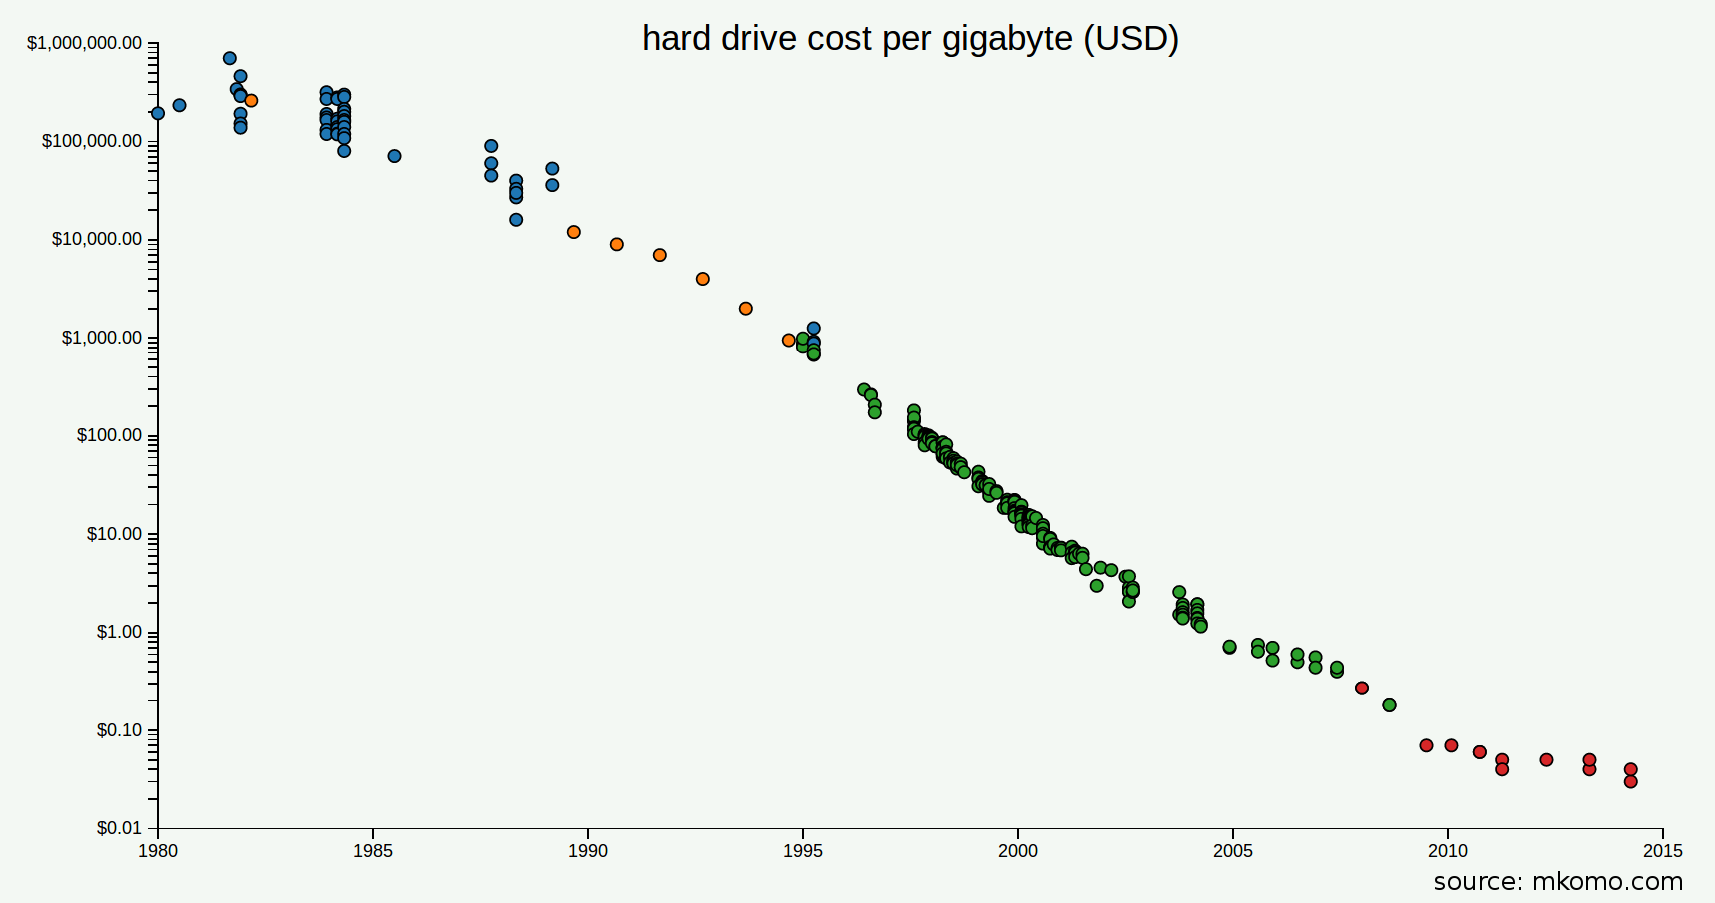
\includegraphics[width=\linewidth]{gfx/hdd-cost-per-gigabyte-large}
    \caption{HDD cost/GB vs. year \citep{hddcost}. \unit[1]{TB} HDD introduced 2007 \citep{first1tb}, \unit[1.5]{TB} introduced 2008 \citep{firsthdd}.}\label{fig:hddcost}
\end{figure}
HDD durability has been maintained despite the cost drop and storage increase  , such that a typical portable USB HDD has a 3-5 year warranty. 
Test results by global leaders in HDD storage have repeatedly shown that consumer HDDs are sufficiently robust for many geoscience storage tasks, as long as proper backup procedures are in place.
Figure~\ref{fig:hddreliability} shows recent HDD reliability under rigorous real-world controlled testing.
\begin{figure}
    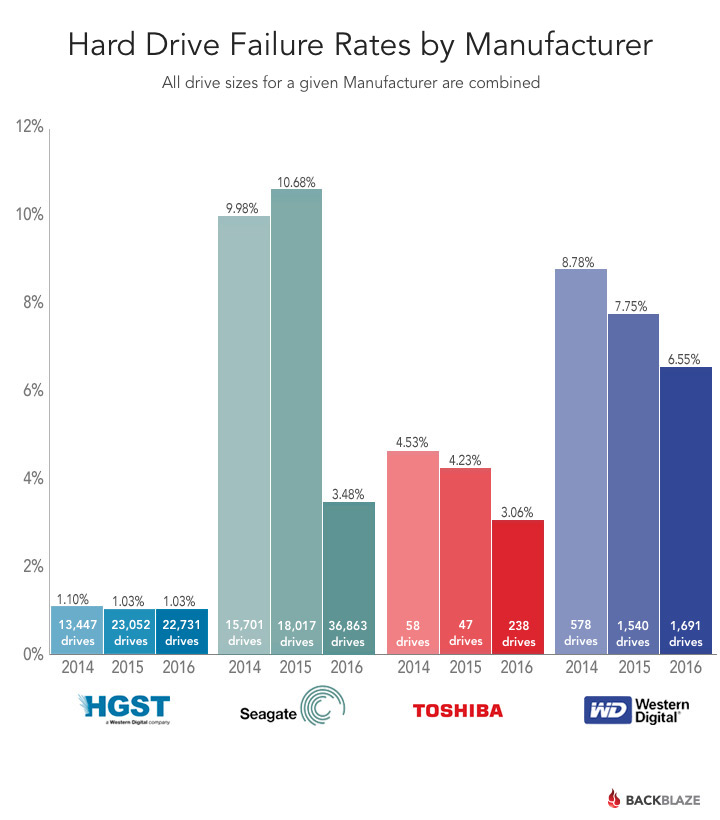
\includegraphics[width=\linewidth]{gfx/drive-stats-2016-q1-failure-by-mfg}
    \caption{Failure rate of large number of continuously used HDD \citep{backblaze2016}.}\label{fig:hddreliability}
\end{figure}
HDD data loss by UAF collaborators has been experienced on some dates HiST was used.
When interesting auroral video is identified, it is copied to multiple drives and when possible the very best snippets are prompted uploaded to Google Drive and other robust cloud storage to help avoid complete data loss.
Figure~\ref{fig:tapeloss} shows file loss experienced on a very large data storage project.
This loss was experienced on high reliability tape drives in a carefully monitored system, and so might be thought of as an example of a practical upper bound on data reliability.
\begin{figure}
    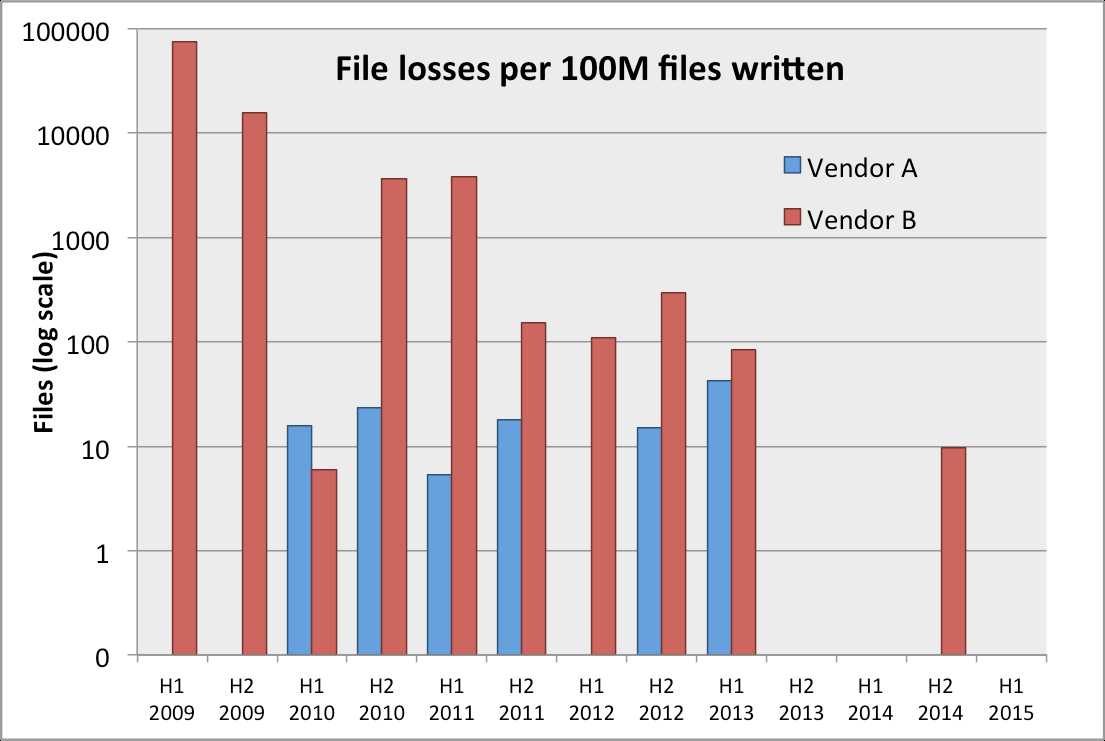
\includegraphics[width=\linewidth]{gfx/tapeloss}
    \caption{Data loss experienced by CERN high reliability storage system \citep{cancio2015}.}\label{fig:tapeloss}
\end{figure}

An example of a leading enterprise HDD \citep{first10tb} is the \unit[10]{TB} Seagate Ironwolf ST10000NE0004 \citep{ironwolf} currently available for \$479.
A five year warranty with \unit[300]{TB/year} write rating exceeds the expected \unit[265]{TB/year} raw data written from a single camera.
As an enterprise HDD, the Ironwolf full-time $24\times7$ failure rate is 0.73\%, substantially better than the consumer HDD of Figure~\ref{fig:hddreliability}.
The sustained data rate specification of \unit[214]{MB/s} is better than some solid state drives (SSD), and is fast enough to handle $2\times2$ binned Andor Neo sCMOS $2560\times2160$ pixel video streaming.
The HDD buffer memory of \unit[256]{MB} is enough to hold
\begin{equation}
256 / \unit[512^2]{pixels} \times \unit[2]{bytes/pixel} \times \unit[56]{frames/s} = \unit[8.7]{s}
\end{equation}
of full frame-rate EMCCD video, a generous margin for operating system hiccups or isolated fragmentation, considering that the HiST program has a RAM pseudocircular buffer as well.

Banks of USB~3.0 external HDD are used for on-site archiving, and may be swapped yearly or as desired if too much data to send over the broadband cellular modem exists.
Assuming Alfvénic or other interesting aurora occurs no more than 10\% of recorded hours, four USB~3.0 HDD at $< \$2000$ total cost are sufficient to store a year's worth of interesting auroral data.
Sections~\ref{sec:obshistory} and~\ref{sec:prochistory} detail the problems solved by industrial technological process and aeronomers to make the next decade one of significant progress in synchronized auroral/ionospheric observations.
Section~\ref{sec:discalgo} describes the DSAD algorithm necessary to process manageable amounts of data, as the full HiST inversion process of chapter~\ref{chapter:sim} is too time-consuming to run on every single frame of data using a single desktop PC. 
If large amounts of data (too much for a single desktop PC) were deemed interesting, computing clusters such as SCC would be very amenable to parallel processing the HiST data inversion.
